\documentclass[12pt, twoside]{article}
\usepackage[francais]{babel}
\usepackage[T1]{fontenc}
\usepackage[latin1]{inputenc}
\usepackage[left=7mm, right=7mm, top=5mm, bottom=5mm]{geometry}
\usepackage{float}
\usepackage{graphicx}
\usepackage{array}
\usepackage{multirow}
\usepackage{amsmath,amssymb,mathrsfs}
\usepackage{soul}
\usepackage{textcomp}
\usepackage{eurosym}
 \usepackage{variations}
\usepackage{tabvar}


\pagestyle{empty}

\begin{document}


\section*{\center{Devoir maison 6}}

\medskip




\begin{center}
\fbox{

\textit{Devoir � rendre sur feuille grand format pour 
\textbf{mardi 9 avril 2013}.}

}
\end{center}

\enskip

\ul{Exercice 1}: \textit{(3 points)}


\begin{enumerate}
  \item D�terminer le PGCD de 1394 et 255. Expliquer votre m�thode.
  \item Un artisan dispose de 1394 graines d'a�a� et de 255 graines de palmier
  p�che. Il veut r�aliser des colliers identiques, contenant chacun le m�me
  nombre de graines d'a�a� et le m�me nombre de graines de palmier p�che.
  
  \begin{enumerate}
    \item Combien peut-il r�aliser au maximum de colliers en utilisant toutes
    ses graines?
    \item Dans ce cas, combien chaque collier contient-il de graines d'a�a� et
    de graines de palmier p�che?
\end{enumerate}

\end{enumerate}

\bigskip

\ul{Exercice 2}: \textit{(5,5 points)}

\enskip


\begin{tabular}{cc}
\begin{minipage}{11cm}
\begin{enumerate}
  \item Reproduire le tableau et compl�ter chaque case par
  \textit{oui} ou \textit{non}.
  \item D'apr�s ce tableau, les fractions $\dfrac{774}{1035}$ et
  $\dfrac{322}{774}$ sont-elles irr�ductibles? Justifier chaque r�ponse.
 
\end{enumerate}
\end{minipage}
&
\begin{minipage}{7,5cm}
\begin{center}
\begin{tabular}{|l|c|c|c|c|}
\hline
\quad & 2 & 3 & 5 & 9 \\
\hline
1035 est divisible par & \quad & \quad & \quad & \quad \\
\hline
774 est divisible par & \quad & \quad & \quad & \quad \\
\hline
322 est divisible par & \quad & \quad & \quad & \quad \\
\hline
\end{tabular}
\end{center}
\end{minipage}
\end{tabular}


\quad \quad 3. D'apr�s ce tableau, peut-on dire que la fraction
  $\dfrac{322}{1035}$ est irr�ductible?
  
 \enskip
  
\quad \quad 4. Calculer le PGCD de 322 et 1035. 


\enskip

\quad \quad 5. La fraction $\dfrac{322}{1035}$ est-elle irr�ductible?  



\bigskip

\ul{Exercice 3}: \textit{(5 points)}

\enskip

\textit{L'unit� de longueur est le centim�tre.}


 ABCD est un carr� tel que AB=4.
Le point M est situ� dans le carr� ABCD et v�rifie AM=2,4 et DM=3,2.
La droite (AM) coupe la demi-droite [DC) au point I.

\begin{enumerate}
  \item Faire une figure.
  \item Montrer que le triangle AMD est rectangle en M.
  \item Calculer au degr� pr�s la mesure de l'angle $\widehat{DAM}$.
  \item Dans le triangle ADI, exprimer $tan (\widehat{DAI})$. En d�duire une
  valeur approch�e au mm pr�s de la longueur DI.
\end{enumerate}
\bigskip

\ul{Exercice 4}: \textit{(5 points)}


\begin{tabular}{cc}
\begin{minipage}{13cm}
Sur la figure ci-contre: $\widehat{ADB}$=52�, BC=20 dm et $\widehat{BDC}$=8�.

\enskip

Calculer le p�rim�tre du triangle ACD arrondi au d�cim�tre. Justifier.
\end{minipage}
&
\begin{minipage}{5cm}
\begin{center}
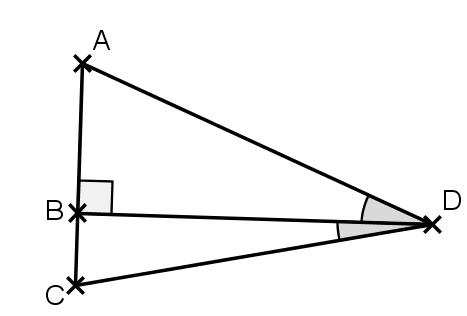
\includegraphics[width=4cm]{images/ex4.png}
\end{center}
\end{minipage}
\end{tabular}
\bigskip

\ul{Exercice 5}: \textit{(2,5 points)}

Dans un triangle rectangle en C, on sait que  $cos$ $\widehat{ABC}$ = 0,8.

\begin{enumerate}
  \item Calculer $(sin$ $\widehat{ABC})^2$ et en d�duire $sin$ $\widehat{ABC}$.
  \item Calculer $tan$ $\widehat{ABC}$
\end{enumerate}
\end{document}
